\hypertarget{coreapi_AQL}{}\section{Core Runtime Support for
AQL}\label{AQL}
AQL is a command-interface for describing a dispatch or a dependency
in a standard format for the queue packet processor. 
To match with and support the AQL packet definitions in the HSA SAR,
HSA core base runtime includes structures for different types of AQL
packets.  SAR defines three different kinds of AQL packets: invalid,
dispatch and barrier.  There is a common packet header across these
three packet types and is defined by the following structure:

\input{STRaql_header}

The \texttt{acquire\_fence\_scope} is used to control the ordering
of memory operations before the packet enters the active state.
There are 4 possible values for acquire fence scope. Each of the
values defines a particular action by HSA agents and components. The
details are described in Table~\ref{acquirefencescope}.

\begin{table}
  \begin{center}
          \begin{tabular}{|p{1in}|p{5in}|}
      \hline
      \textbf{Acquire Fence Scope} &\textbf{Description} \\ 
      \hline
      0	& None -- no fence is applied. \\
      \hline
      1	& Make memory operations made by this HSA component prior to
      launch of this packet, visible to this packet operation.\\
      \hline
      2	& Make memory operations made by HSA agents prior to launch
      of this packet, visible to this packet operation.\\
      \hline
      3	& Make memory operations made by HSA agents prior to launch
      of this packet, visible to this packet operation, and affected
      caches in the HSA Component are invalidated.\\
      \hline
    \end{tabular}
  \end{center}
  \caption{Acquire Fence Scope Values and Actions}
  \label{acquirefencescope}
\end{table}

Similarly, the release fence scope, which is also 2 bits, can be
used to define the desired memory fence and cache actions at the
end of kernel execution, but prior to the packet being marked as
complete. Table~\ref{releasefencescope} describes the different
controls.

\begin{table}
  \begin{center}
          \begin{tabular}{|p{1in}|p{5in}|}
      \hline
      \textbf{Release Fence Scope} &\textbf{Description} \\ 
      \hline
      0	& None -- no fence is applied. \\
      \hline
      1	& The release fence is applied to the HSA Component only. \\
      \hline
      2	& The release fence is applied globally to the HSA System.\\
      \hline
      3	& The release fence is applied globally to the HSA System,
      and additionally affected caches in the HSA Component are
      cleaned and invalidated.\\
      \hline
    \end{tabular}
  \end{center}
  \caption{Release Fence Scope Values and Actions}
  \label{releasefencescope}
\end{table}

The \texttt{format} field in the header is used to specify
the packet type. Beyond the three packet types defined, all the
other packet types are reserved for implementation use. In addition
to this, the last 15 bits in the packet header are also reserved for
future or implementation specific use. The format field indicates
the type of the packet. Of the three packet types, the
dispatch and the barrier packet have individual packet-state
diagrams that are discussed along with their description.

\paragraph{Invalid AQL packet} Indicates that the packet not ready
to be processed by the packet processor. 

\hypertarget{dispatch_packet}{}\subsection{Dispatch AQL
Packet}\label{dispatch_packet}

Dispatch packet type is used for dispatching a kernel on to a HSA
component.  The dispatch AQL packet can have five different states:
\emph{on queue}, \emph{processing}, \emph{error}, \emph{active} or
\emph{complete}. Figure~\ref{fig:packetstate} shows the different
states of a packet and transitions leading to those states.

\begin{figure}
  \centering
  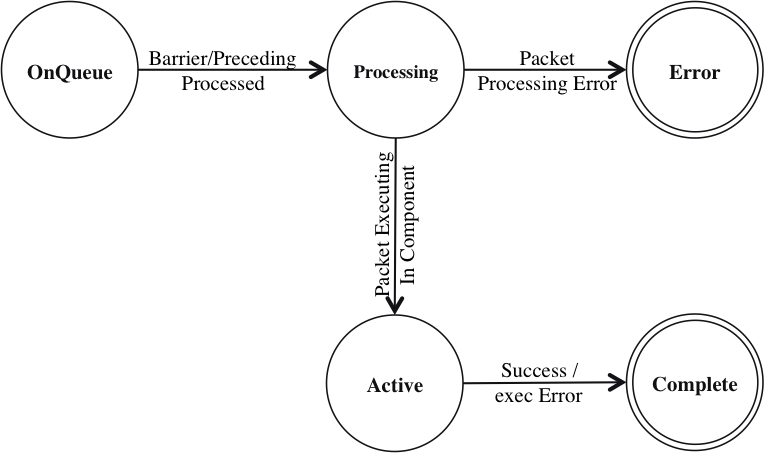
\includegraphics[width=0.5\textwidth] {packetstate}
  \centering
  \caption{Dispatch Packet State Diagram}
  \label{fig:packetstate}
\end{figure}

\begin{description}
\item[On queue state] A packet is considered to in the on queue
state once the format of the packet is changed from invalid (a value
of 0) to a value of 1 or 2. Any other value for format puts the
packet and the queue in error state.

\item[Processing state] If this dispatch packet has the barrier bit
set, then the processing of this packet occurs only after all prior
kernels have completed execution.  Otherwise, once the packets prior
to this packet are processed, the packet processor begins to process
this packet and the packet enters the processing state.  From the
launch state, two states are possible: error or active.

\item[Error state] the packet processor encountered an error
processing this packet. This results in a queue error (see
Figure~\ref{fig:queuestate}) and the packet enters the error state
(the completion object is signaled with error by the packet
processor). The following errors are indicated via an error signaled
to the completion object: 
processing parsing error, dependency resolution error, system error
and premature termination due to queue inactivation.
When the user invokes the
\ttbf{hsa\_queue\_force\_deactivate} API or the
\ttbf{hsa\_queue\_destroy} API while the packet is this state, the
completion object will be signaled with error.

\item[Active state] If the packet processing is successful and the
kernel the packet represents is either executing or queued for
execution, the packet enters the active state. From active state,
either successful or failed execution both take the packet into the
completed state.  Alternatively, a user action (see
~\ref{queue_force_deactivate}) can also take the packet out of
active state into complete state.  When the user invokes the
\texttt{hsa\_queue\_force\_deactivate} API or the
\texttt{hsa\_queue\_destroy} API while the packet is this state, the
completion object will be signaled with error. 

\item[complete state] A packet enters a complete state after its
completion signal is signaled (either with success or failure).
\end{description}

A dispatch packet is considered processed once the packet processor
processes it and makes the queue slot occupied by this packet
available. A processed dispatch packet may endure a period of time
where it is awaiting its dispatch on to the HSA component. Even such
packets awaiting execution are still considered as processed. 

The structure for the dispatch AQL packet is shown below:

\input{STRdispatch_packet}

\hypertarget{segment_sizes}{}\subsubsection{Segment
Sizes}\label{segment_sizes}
If the kernel being dispatched uses private and group segments, the
user is required to specify the sizes of these segments in the AQL
dispatch packet. Manually calculating this information is not 
feasible and requires visual inspection of the user program, which itself
may have been generated by a higher-level compiler. Hence the user
must rely on the \texttt{finalizer} to get the corresponding segment
sizes. Further details about determining segment sizes described in
Section~\ref{coreapi_finalizer_overview}. 

Of the other HSA segments, the kernarg segment is also a part of
the AQL packet, but as a pointer. This is because kernarg segment
carries the arguments required to execute the kernel being
dispatched and must be setup by the user (as specified in
Section~\ref{coreapi_HSAIL_ABI}) prior to writing the AQL packet to
the queue (unlike the group and private segments, whose lifespan
spans only the active state of the AQL dispatch packet).

\hypertarget{barrier_packet}{}\subsection{Barrier AQL
packet}\label{barrier_packet} 
The barrier packet allows the user to specify up to 5 dependencies
as \texttt{hsa\_signal} objects and require the packet processor to
resolve them before proceeding. The barrier packet is a blocking
packet, in that the processing of the barrier packet
\emph{completes} the packet and its completion object is signaled.
This is unlike a dispatch packet whose completion may occur at some
future time after the packet has finished processing. The HSA core
base runtime structure for the AQL barrier packet is shown below:

\input{STRbarrier_packet}

If any of dependent signals have been signaled with a negative
value, the barrier packet is complete, and will indicate failure in
its completion signal. The \texttt{completion signal} will be
signaled with the error value as discussed in
Section~\ref{signal_error}.

If the queue is not already in an error state (e.g. the job
generating the error was processed in a different queue) then the
HSA Packet Processor should consider the error code on the dependent
signal to indicate an error in the queue itself and subsequently
signal the \texttt{error\_signal} in the queue.

When all of the dependent signals have been signaled with the value
0, the \texttt{completion\_signal} will be signaled with the value 0 to
indicate a successful completion.

The barrier packet also has a barrier bit that indicates that this
packet may only be processed when all previous packets have been
marked as completed.

Alike the dispatch packet, the barrier packet can also be in one of
the following states: \emph{on queue}, \emph{processing},
\emph{completed, error} or \emph{completed, success}.

\begin{description}

\item[On queue state] A packet is considered to in the on queue
state once the format of the packet is changed from invalid (a value
of 0) to a value of 1 or 2. Any other value for format puts the
packet and the queue in error state.

\item[Processing state] If this barrier packet has the barrier bit set,
then the processing of this packet occurs only after all prior
dispatch packets have completed execution.  Otherwise, once the
packets prior to this packet are processed, the packet processor
begins to process this packet and the packet enters the processing
state.  From the launch state, two states are possible: completion,
error or completion, success.

\item[completed-error] The barrier packet reaches this state from
the processing state if (a) one of the dependency signals had an
error, and (b) if the packet was malformed (e.g. bad signal object
or invalid usage of reserved bits). A barrier packet can also reach
this state when the user invokes the
\texttt{hsa\_queue\_force\_deactivate} API or the
\texttt{hsa\_queue\_destroy} API while the packet is in processing
state (the completion object will be appropriately signaled with an
error).

\item[completed-success] The barrier packet had all its dependencies
met, its completion object has been signaled with a value of 0.

\end{description}

\begin{figure}
  \centering
  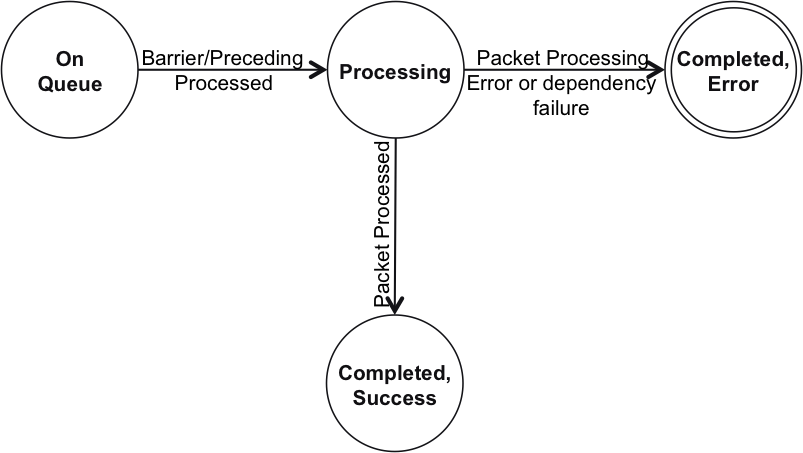
\includegraphics[width=0.5\textwidth] {barrierpacketstate}
  \centering
  \caption{Barrier Packet State Diagram}
  \label{fig:barrierpacketstate}
\end{figure}

A state diagram in Figure~\ref{fig:barrierpacketstate} shows these
transitions.

\hypertarget{aql_example}{}\subsection{AQL Setup
Example}\label{aql_example}


